\section{Results}
\paragraph{}
In this section the results of the experiments preformed as part of the project. The results will be presented per application and, if required, are divided into several test runs if required. The tests have been performed several times. The experiment have been performed on both the virtual and hardware environment.

\subsection{Paessler Webserver Stress Tool}
The experiment has been preformed multiple times, with the same scenario. Afer each experiment the database referted the original state. Each user has made multiple requests to a balanced set of application functions, based on the shopping scenario, triggering different kind of transactions. Requests got timed-out after about 1500ms. A scenario to simulate realistic transactions on the full-setup webshop. Has been preformed using the steps shown in \textbf{figure \ref{fig:pto1}}, \textbf{figure \ref{fig:pto2}} and \textbf{figure \ref{fig:pto3}} shown below. An example of such scenario script can be found in Appendix 3 (listening \ref{Appendix3}).

 \begin{figure}[H]
    \centering
    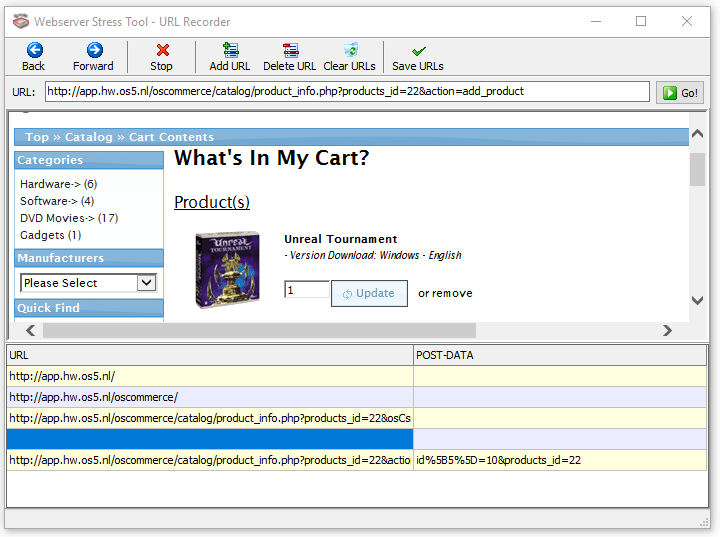
\includegraphics[width=9cm]{Pictures/pto01.PNG}
    \caption{URL recording}
    \label{fig:pto1}
\end{figure}

 \begin{figure}[H]
    \centering
    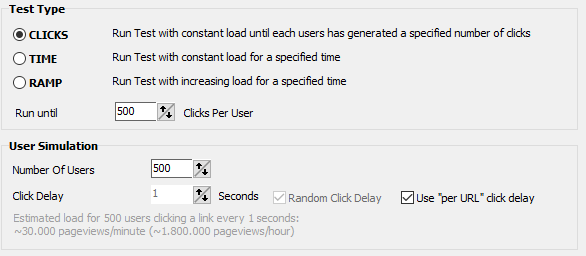
\includegraphics[width=8cm]{Pictures/pto02.PNG}
    \caption{Test characteristics and userdelay}
    \label{fig:pto2}
\end{figure}

 \begin{figure}[H]
    \centering
    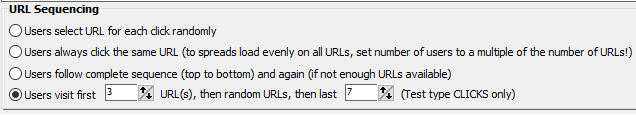
\includegraphics[width=8cm]{Pictures/pto03.PNG}
    \caption{URL sequencing}
    \label{fig:pto3}
\end{figure}
\clearpage
\subsubsection{Result: Measuring requests \& transferred data}
\paragraph{}
First the result of the request and transferred data are shown below. The hardware in \textbf{figure \ref{fig:resP1hw}}  and for the VM we refer to \textbf{figure \ref{fig:resP1vm}} which show the number of open requests as well as the number of sent and received requests in comparison with the network traffic on both the virtual and physical setups.

 \begin{figure}[H]
    \centering
    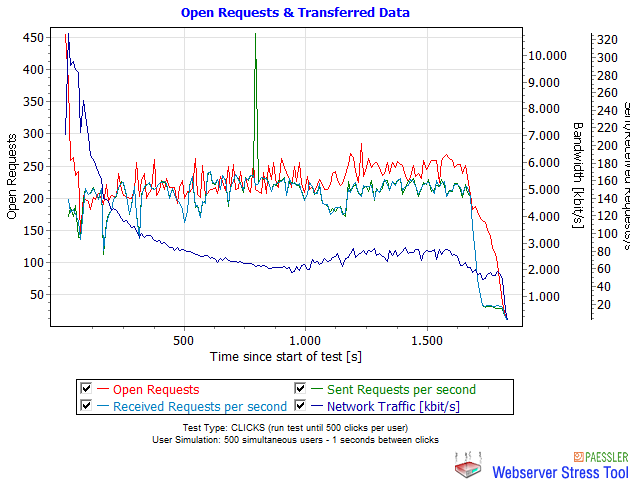
\includegraphics[width=10cm]{Pictures/graph6hw.png}
    \caption{Requests \& Transferred Data for Physical Setup}
    \label{fig:resP1hw}
\end{figure}

\begin{figure}[H]
    \centering
    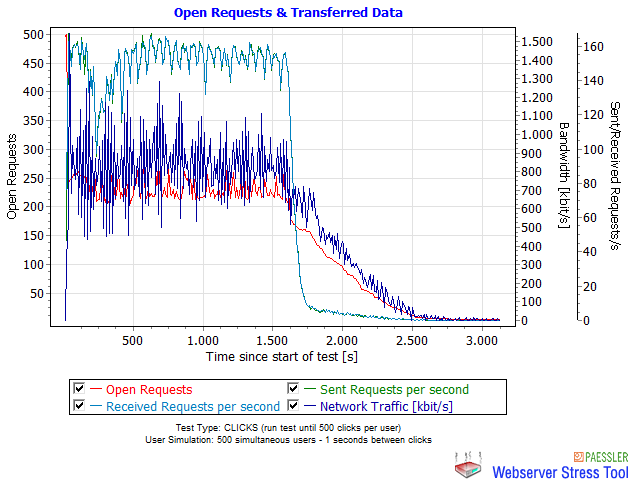
\includegraphics[width=10cm]{Pictures/graph6vm.png}
    \caption{Requests \& Transferred Data for Virtual Setup}
    \label{fig:resP1vm}
\end{figure}

\paragraph{}
The 500 users we nicely balanced in the hardware setup, while on the virtual setup they were handled all at the same time. A large amount of requests on the virtual setup timed-out before they were handled by web server. 

\subsubsection{Result: Measuring transferred Data \& system Memory \& CPU load}
\paragraph{}
The second result is about the transferred data. Below in \textbf{figure \ref{fig:resP2hw}} for the hardware and for the VM we refer to \textbf{figure \ref{fig:resP2vm}}, which describe the measurement for vital parameters of the machine it runs on. It can be helpful to find out if the limits of the test client have been reached testing both the virtual and physical setups:

 \begin{figure}[H]
    \centering
    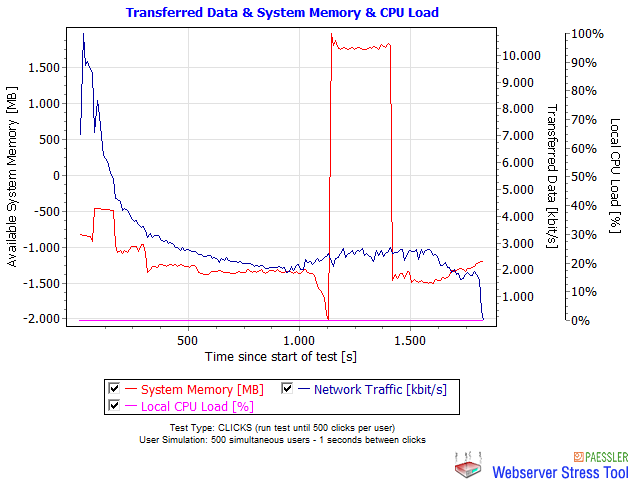
\includegraphics[width=10cm]{Pictures/ph1.png}
    \caption{Transferred Data \& System Memory \& CPU Load for Physical Setup}
    \label{fig:resP2hw}
\end{figure}
   
 
\begin{figure}[H]
    \centering
    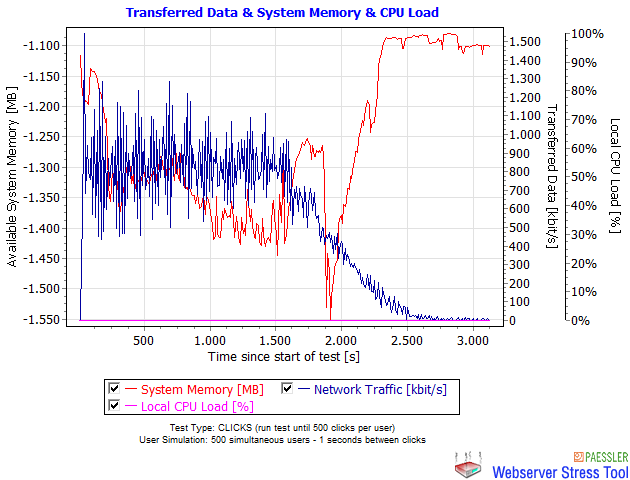
\includegraphics[width=10cm]{Pictures/vm1.png}
    \caption{Transferred Data \& System Memory \& CPU Load for Virtual Setup}
    \label{fig:resP2vm}
\end{figure} 

\paragraph{}
The 500 users on the hardware setup are handled smoothly in order. There is a continuous rate of requests handled by the server. During the experiment on the virtual setup there was much more requests queued in memory. The response were handled two seconds later by the client.

\subsubsection{Result: Measuring Click Time, Hits/s \& Clicks/s}
\paragraph{}

\textbf{Figure \ref{fig:resP3hw}} \& \textbf{figure \ref{fig:resP3vm}} illustrate the average time a user waited for his request to be processed (including redirects, images, frames, etc., if enabled), the hits per second, and the users per clicks. 

 \begin{figure}[H]
    \centering
    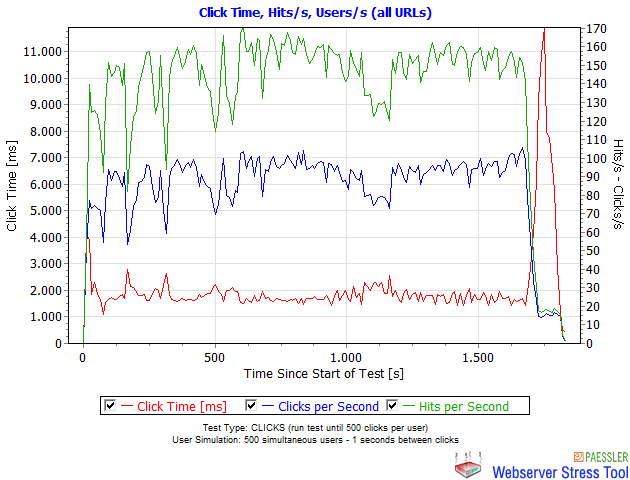
\includegraphics[width=10cm]{Pictures/ph2.png}
    \caption{Click Time, Hits/s \& Clicks/s for Physical Setup}
    \label{fig:resP3hw}
\end{figure}
   
 
\begin{figure}[H]
    \centering
    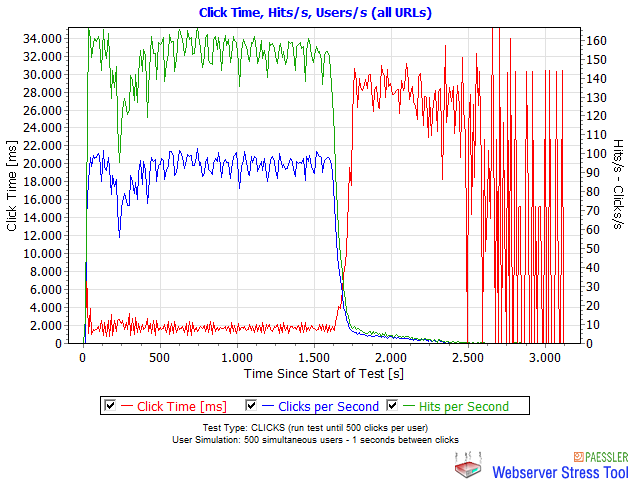
\includegraphics[width=10cm]{Pictures/vm2.png}
    \caption{Click Time, Hits/s \& Clicks/s for Virtual Setup}
    \label{fig:resP3vm}
\end{figure} 


\paragraph{}
We can see that with 500 users the two lines for “clicks per second” (blue) and “hits per second” (green) differ more and more. The reason is that hits includes requests that produce errors, but clicks are only calculated from the requests that were successful.

\subsection{Apache Benchmark}

\begin{itemize}
    \label{abtestbul}
    \item Test 1: Full-Setup
    \begin{itemize}
        \item A load of similar transactions on the full-setup webshop.
        \item Due to the nature of the webshop, the responses are slightly used specific. Because functions like the shoppingcart-session.
        \item Generates multiple read and write transactions to the database.
        \item Makes use of a round-robin load balancing reverce proxy based on ngnix.  
    \end{itemize}
    \item Test 2: Webserver-only
    \begin{itemize}
        \item A load of similar transactions on apache webserver only.
        \item Generates multiple requests for a specific resource.
        \item Does not make use of the proxy and/or the database.
    \end{itemize}
    \item Test 3: Optimized CPU and Memory
    \begin{itemize}
        \item A combination of test 1 and 2 with a optimized CPU and memory mix.
    \end{itemize}
\end{itemize}

\subsubsection{Test 1: Full-Setup}
Test with AB to Proxy displayed in \textbf{figure \ref{fig:resA1hw}} \& \textbf{figure \ref{fig:resA1hw}}. As described in the bullets above \textit{(\ref{abtestbul})}.
The first experiment uses 4 servers and the target is the catalog of the webshop at the proxy server.

 \begin{figure}[H]
    \centering
    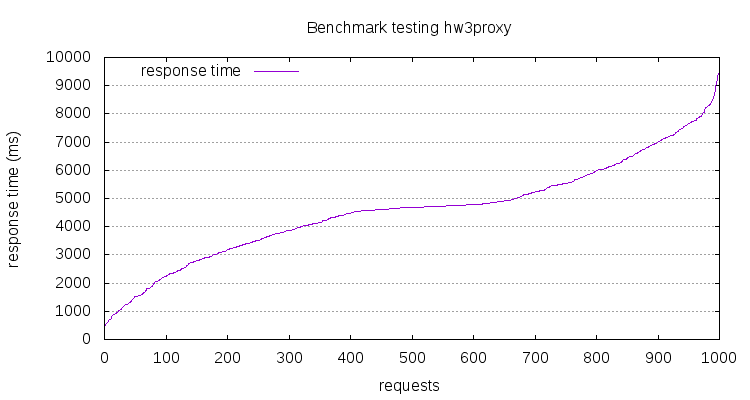
\includegraphics[width=10cm]{Pictures/abresult_hw_1.png}
    \caption{Test 1: Full-Setup for Physical Setup}
    \label{fig:resA1hw}
\end{figure}
\begin{figure}[H]
    \centering
    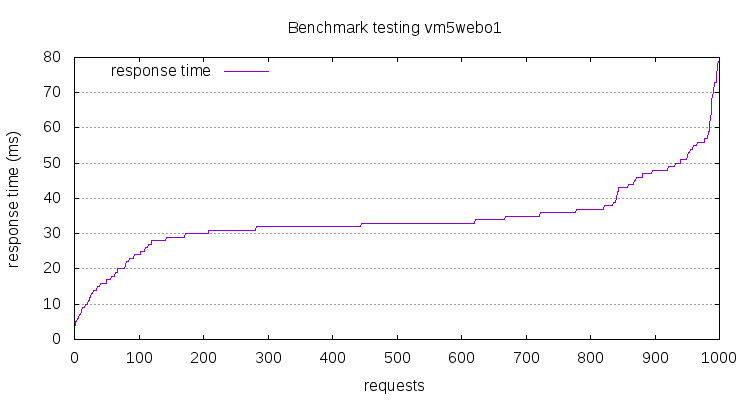
\includegraphics[width=10cm]{Pictures/abresult_vm_2.png}
    \caption{Test 1: Full-Setup for Virtual Setup}
    \label{fig:resA1hw}
\end{figure} 

\subsubsection{Test 2: Webserver-only}
Test with AB to Webserver displayed in \textbf{figure \ref{fig:resA2hw}} \& \textbf{figure \ref{fig:resA2hw}}. As described in the bullets above \textit{(\ref{abtestbul})}.
The second test has been preformed to test the server without the application, database transactions and calculations.

 \begin{figure}[H]
    \centering
    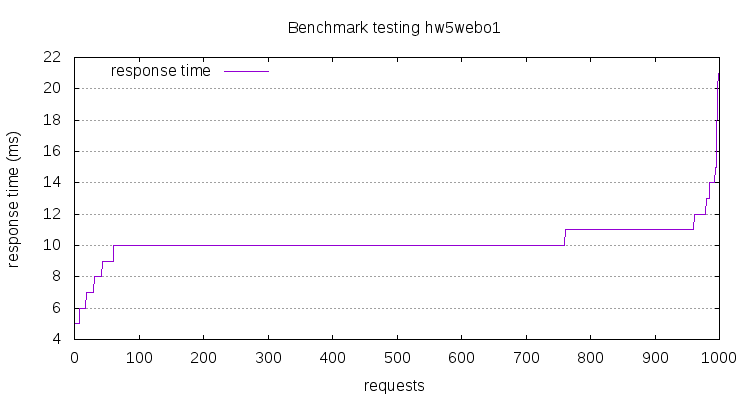
\includegraphics[width=10cm]{Pictures/abresult_hw_2.png}
    \caption{Test 2: Webserver-only setup for Physical Setup}
    \label{fig:resA2hw}
\end{figure}
   
 
\begin{figure}[H]
    \centering
    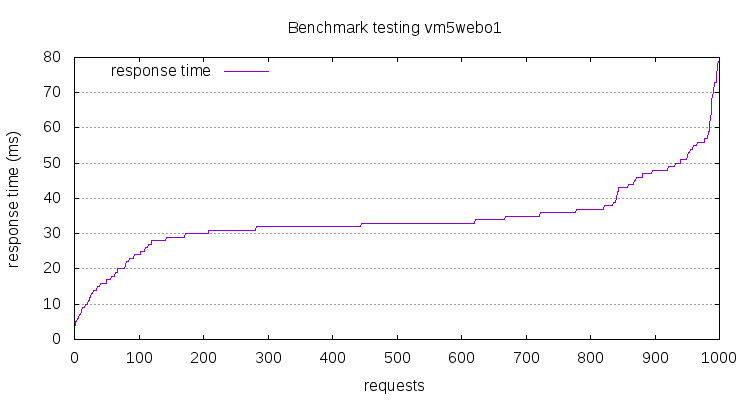
\includegraphics[width=10cm]{Pictures/abresult_vm_2.png}
    \caption{Test 2: Webserver-only setup for Virtual Setup}
    \label{fig:resA2hw}
\end{figure} 
\clearpage
\subsubsection{Test 3: Optimized CPU and Memory}
Test with optimized CPU and Memory, with both setup, on the VM. Seen in \textbf{figure \ref{fig:resA3vm2}} \& \textbf{figure \ref{fig:resA2hw}}. As described in the bullets above \textit{(\ref{abtestbul})}. The last test has been preformed to see the inpact of the configuration.
 \begin{figure}[H]
    \centering
    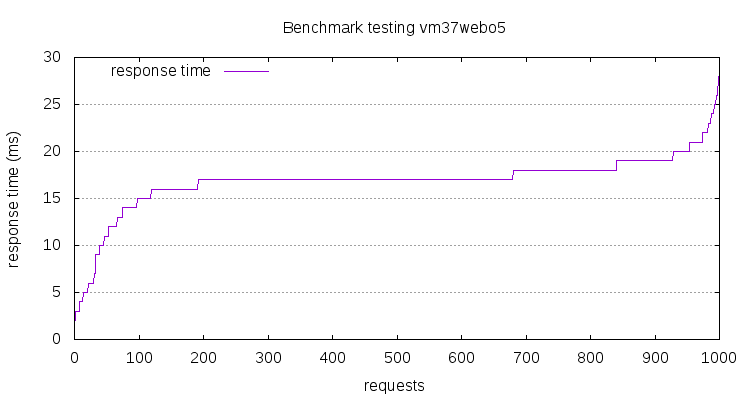
\includegraphics[width=10cm]{Pictures/abresult_vm_3a.png}
    \caption{Test 3: Optimized CPU and Memory setup for Full VM Setup}
    \label{fig:resA3vm1}
\end{figure}
   
\begin{figure}[H]
    \centering
    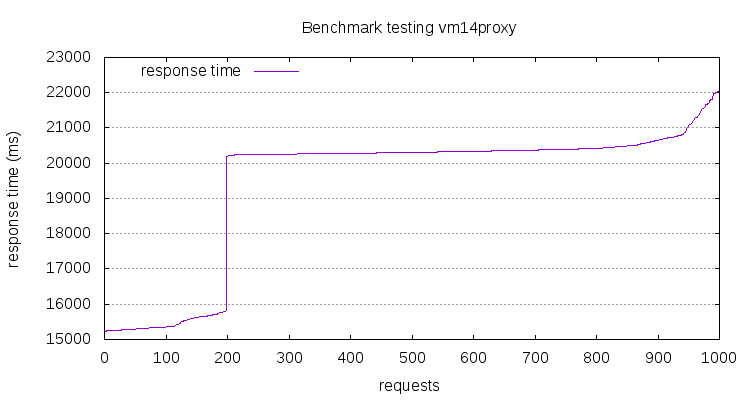
\includegraphics[width=10cm]{Pictures/abresult_vm_3b.png}
    \caption{Test 3: Optimized CPU and Memory setup for Web-only VM Setup}
    \label{fig:resA3vm2}
\end{figure} 